\documentclass[12pt,a4paper,titlepage]{report}
\usepackage[utf8]{inputenc}
\usepackage[T1]{fontenc}
\usepackage{amsmath}
\usepackage{amssymb}
\usepackage{graphicx}
\usepackage{cite}
\usepackage{subcaption}
\graphicspath{ {./figures/} }

\newcommand{\citeme}[0]{\textbf{\emph{CITEME}}}
\newcommand{\todo}[1]{\textbf{\emph{TODO: } #1}}

\usepackage{titlesec}

\titleformat{\chapter}[display]{\normalfont\bfseries}{}{0pt}{\Huge}


\begin{document}
	\begin{titlepage}
		\centering\Large\emph{Electronics and Computer Science Faculty of Engineering and Physical Sciences University of Southampton}
		\\[2cm]
		\centering\Large{Josh Pattman} \\
		\centering\Large{12 December 2022} \\
		\centering\huge\textbf{Investigating Optimisations Of Swarm Learning With Respect To Real World Challenges}
		\\[2cm]
		\centering{\large{Project Supervisor:} \linebreak \Large{Dr Mohammad Soorati - \emph{m.soorati@soton.ac.uk}}} \\[1cm]
		\centering{\large{Second Examiner:} \linebreak \Large{Dr Jo Grundy - \emph{j.grundy@soton.ac.uk}}}
		\\[2cm]
		\centering\Large{A project progress report submitted for the award of \textbf{Computer Science with Artificial Intelligence}}
	\end{titlepage}

	\chapter*{Statement of Originality}
\begin{itemize}
	\item I have read and understood the ECS Academic Integrity information and the University’s
	Academic Integrity Guidance for Students.
	\item I am aware that failure to act in accordance with the Regulations Governing Academic Integrity
	may lead to the imposition of penalties which, for the most serious cases, may include
	termination of programme.
	\item I consent to the University copying and distributing any or all of my work in any form and
	using third parties (who may be based outside the EU/EEA) to verify whether my work
	contains plagiarised material, and for quality assurance purposes.

	\item I have acknowledged all sources, and identified any content taken from elsewhere.
	\item I have not used any resources produced by anyone else.
	\item I did all the work myself, or with my allocated group, and have not helped anyone else.
	\item The material in the report is genuine, and I have included all my data/code/designs.
	\item I have not submitted any part of this work for another assessment.
	\item My work did not involve human participants, their cells or data, or animals.

\end{itemize}


	\chapter*{Abstract}	
	Federated learning is a technique that allows a machine learning model to be trained on data distributed across multiple data islands without ever sharing the data. This approach protects privacy by keeping the data decentralized. Swarm learning is a similar technique that eliminates the need for a central server, ensuring that not only the data, but also the communication, is completely decentralized. The goal of this project is to design and implement a swarm learning algorithm, then test the algorithm in multiple scenarios inspired by the real world. The algorithm will then be evaluated against other machine learning techniques to investigate if swarm learning is a viable technology for the modern world.

	\tableofcontents
	\chapter{Background and Literature Review}
\section{Background Research}
\subsection{Keras and Python}
What i did to learn keras and python and prepare myself
\subsection{Iridis 5}
What i did to learn about using iridis 5 and prep
\section{Literature Review}
\subsection{A survey on federated learning \cite{survey_on_fed_learning}}
This paper is a good introductory piece to the field of federated learning. It covers a wide range of topics, without going into too much detail, which was useful to direct the author into reading more specific papers. The paper also has a basic introduction to how federated learning works, and also some potential use cases for federated learning. All in all, this paper helped point the author in the right direction for further research.

\subsection{Swarm Learning for decentralized and confidential clinical machine learning \cite{swarm_learning}}
Despite the fact that this paper focusses on a medical use case, it is a good introductory piece to the topic of swarm learning. A theme of the paper is privacy, and how it can affect the training speed of models. The paper points out that due to privacy legislation, sharing data between hospitals is not possibly, which can mean that training machine learning models does not reach an optimal outcome. However, a solution is proposed in the form of swarm learning: effectively a decentralised form of federated learning. It is shown that swarm learning can outperform the models trained at individual hospitals without communication.

The paper also gives a good high level summary of how the swarm learning algorithm works. This was particularly useful in giving the author a basic understanding of swarm learning to prepare for further research.

\subsection {Federated learning in Robotic and Autonomous Systems \cite{fed_in_robotics}}
\begin{itemize}
	\item Introduced to using federated learning in robotics
	\item Real world reasons that federated learning is useful in the field of robotics
	\item Horizontal/vertical federated learning
	\item Brief look at federated object detection
	\item Practical challenges of federated (model upload time, etc)
\end{itemize}

\subsection{Decentralized Federated Learning: A Segmented Gossip Approach \cite{gossip_learning}}
\begin{itemize}
	\item Problem of bandwidth for federated learning
	\item Had a very cool novel idea that every step each node only needs to pull a segment of the network. This reduces bandwidth and should deffo be somthing to try
\end{itemize}

\subsection{Multi-Center Federated Learning \cite{multi_center_fed_learning}}
\begin{itemize}
	\item 
\end{itemize}

\subsection{FedBN: Federated Learning On Non-IID Features via Local Batch Normalization \cite{fedbn}}
\begin{itemize}
	\item 
\end{itemize}

\subsection{Personalized Federated Learning with Theoretical Guarantees: A Model-Agnostic Meta-Learning Approach \cite{model_agnostic_meta_learning}}
\begin{itemize}
	\item 
\end{itemize}
	\chapter{Project Goals}
\section{Problem}
Currently, there is more data stored around the world than ever before. However, there are also many recent regulations that prevent the data from being used by machine learning algorithms. In many cases, this is because the data owners are not comfortable or able to send the data to a central server for processing and training. The result of this is that either each data owner has to train their own inferior models, or no models are trained at all due to the lack of data.

In addition to this, the world also has more electronic devices than ever before. As these devices become more and more powerful, using each device to train a machine learning model on a small amount of data becomes a possibility. However, these devices will still not outperform a fast computer alone.

\section{Proposed Solution}
One of the key features of swarm learning is that data never needs to be shared among the agents in the learning network, which is beneficial for the protection of private data. Given this, swarm learning seems well-suited to the problem at hand. In addition, swarm learning may be able to more effectively utilize the processing power of a network of connected devices. However, swarm learning is still a relatively new algorithm and faces many real-world challenges that have only been addressed individually in existing research.

\section{Goals}
\textbf{To investigate possible optimisations of the swarm learning algorithm on simple problems, whilst adding real world constraints incrementally, and eventually arriving at a robust swarm learning algorithm that addresses many real world issues in one.}

\begin{enumerate}
	\item Create a working implementation on a simple dataset of swarm learning
	\item Incrementally add real world problems to the swarm learning algorithm
	\item Mitigate the effects of the problem on the accuracy of the algorithm by implementing either novel ideas or methods from existing literature.
	\item Ensure that the end product is as reproducible as possible such that it can be re-implemented for specific use cases.
\end{enumerate}
\subsubsection{Problems}
Below are some real world problems with swarm learning. This is not a comprehensive list and more problems could be researched if necessary.
\begin{itemize}
	\item \textbf{Unevenly distributed features/local bias} - This is where feature in the dataset are not distributed evenly between agents. For instance, when classifying mnist, one agent may see more 7s and one may see more 2s.
	\item \textbf{Sparsely connected networks} - This refers to a situation where each agent does not have direct communication with every other agent, but instead can only communicate with a few neighbours.
	\item \textbf{Data transfer limits} - This is a situation where an agent may not be able to send an entire neural network over the internet, due to connection speed.
	\item \textbf{Low processing power agents} - This situation is where agents have much lower processing power than a standard machine that one may train a model on. For example, agents may not have access to a GPU.
\end{itemize}	

\section{Focussing On Project Goals}
The plan for this project went through multiple iterations before the final plan was formulated:
\begin{enumerate}
	\item The initial plan was to \emph{control a swarm of drones to detect objects such as natural disasters or people needing help, whilst also improving accuracy of the model over time}
	\item After discussion, the plan was changed to be \emph{perform edge processing and distributed object detection on many camera perspectives of an environment to decide where disasters are happening, whilst learning to improve the model over time}
	\item Following the initial research phase, the plan was narrowed to \emph{explore ways to optimise swarm learning for distributed detection of a simple abstract object}
	\item Finally, after the second phase of research, the settled upon plan became \emph{Investigate possible optimisations of the swarm learning algorithm}. This is the current plan.
\end{enumerate}
The shift of focus away from object detection and towards swarm learning is mainly for two reasons:
\begin{enumerate}
	\item The author finds the swarm learning aspect of the project to be the most interesting part, especially after researching the subject
	\item A general framework of improvements and algorithms on swarm learning is much more useful to the real world than an implementation on a simple simulation.
\end{enumerate}
	\chapter{Progress of Implementations}

\section{Basic MNIST classifier}
A simple \emph{mnist} classifier was built using \emph{Keras} in \emph{Python}. There was only one agent which trained on the dataset, and the main reason for this was to get a baseline for the swarm learning to compete against.

\section{Simple swarm learning}
Using the same model for each agent as used in the \emph{Basic MNIST classifier}, a swarm of agents was created. Each agent had access to the whole dataset for training. Every agent also could communicate with every other agent. The agents acted in a loop, where they would each first train for one epoch on their copy of the training set, and then would average their models weights with all of their neighbours weights. This implementation consisted of 5 agents. The following graphs showing the multiple agent accuracy show only the accuracy of one agent in the swarm, but all of the agents had similar results.

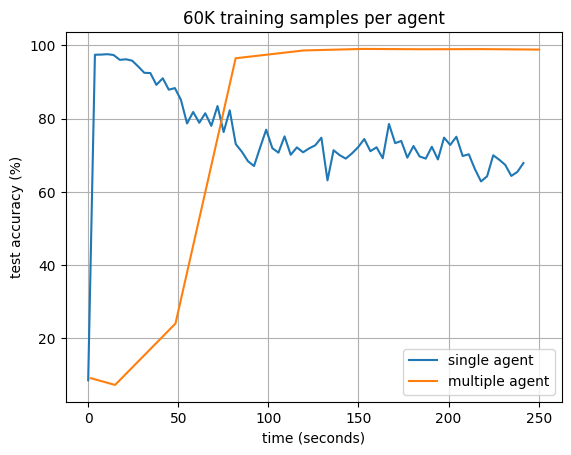
\includegraphics[width=\textwidth]{accuracy_60k}

To start off with, the swarm was a lot slower to increase its accuracy than the single agent algorithm. After some time, the swarm increased in accuracy to the same point as the single agent. However, after reaching this point, the single agent started to overfit but the swarm continued to increase in accuracy. The swam eventually settled upon a higher accuracy than the single agent ever achieved.

The agents seemed to reach the final accuracy in fewer training steps if the agents training loops were offset by even intervals of time. The author hypothesizes that this may be because when the agents training is synced, some of the agents may skip the just completed training when requesting updates, which can cause training epochs to effectively be lost. This effect needs further investigation.

\section{Reduced dataset swarm learning}
This experiment was focussed around reducing the amount of data each agent gets to train on. A number of samples were selected randomly for each agent from the training set, and these never changed throughout training. This test was run for 2000 and 500 samples per agent.

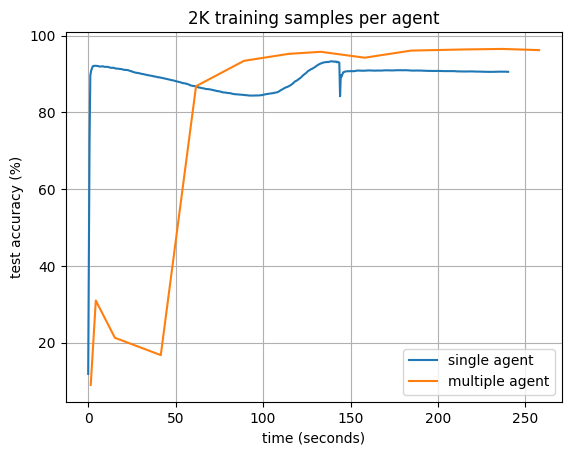
\includegraphics[width=\textwidth]{accuracy_2k}

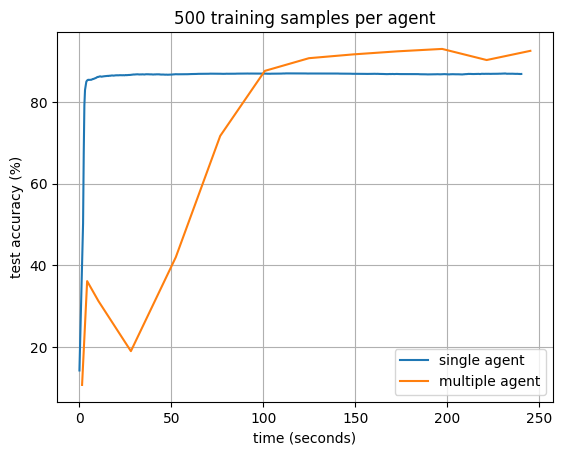
\includegraphics[width=\textwidth]{accuracy_500}

In both cases, the swarm took a lot longer to reach its peak accuracy, nevertheless, the swarm exceeded the peak accuracy of the lone agent by about 5\%-10\%.

On both graphs, there is a spike in accuracy near the start of swarm training, then a reduction in accuracy, then a stable increase. This is caused by new agents with untrained networks joining the swarm and adding effectively a random model to the pool of weights. An easy fix for this would to make an agent that has just joined the network request a model from its neighbours immediately, and use that as a base network. This has not been implemented due to time constraints. 
	\chapter{Project Planning}

\section{Planned Phases of the Project}
The project is divided into several phases, which must be completed in sequence. Throughout these phases, the interim and final reports will be developed concurrently as a skeleton.
\begin{enumerate}
	\item Research - This phase consists of finding and reading existing literature. It is at this time that the project idea is developed fully.
	\item Simple Implementation - In this phase, a proof of concept implementation will be developed. It will entail a simple swarm learning algorithm learning on a basic dataset, without any complex problems. This implementation will be build upon in further phases.
	\item Interim Report - This phase is focussed on filling out and finalising the interim report.
	\item Main development - In this phase, the iterative development of the swarm learning algorithm will occur. This is actually a repetition of four sub-phases:
	\begin{enumerate}
		\item Further research on real-world problem
		\item Implement real-world problem and test current solution
		\item Implement mitigations and test / evaluate
		\item Document any discoveries and evaluations of mitigations
	\end{enumerate}
	\item Final report - In this phase, the final report will be written up.
	\item Housekeeping - This is the final phase which is used for any extra jobs that were not able to be completed in other phases.
\end{enumerate}



\section{Completed Work}
A Gantt chart was created to plan the completion of different sections of the project prior to the interim stage. This chart was closely followed and proved to be a valuable tool for time management. The Gantt chart was developed after the initial project brief was submitted.

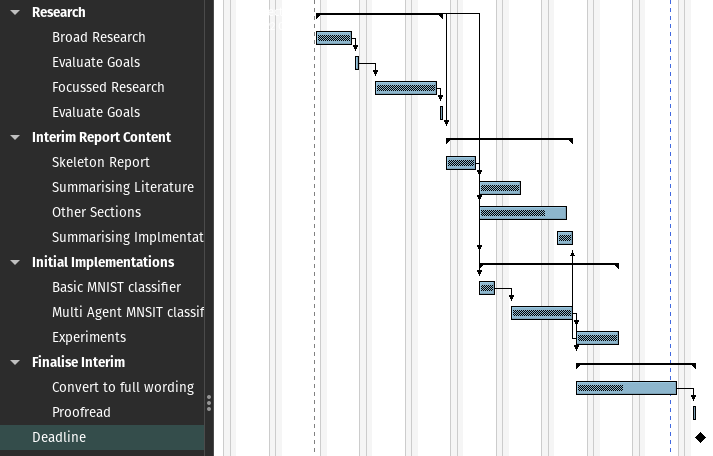
\includegraphics[width=\textwidth]{gantt_pre}


\section{Remaining Work}
A second Gantt chart was created to plan the project after the interim stage. This chart was developed near the end of the first semester, after a more thorough understanding of the project had been obtained through research. The chart only includes plans for two problems, as it was determined that this is the minimum number required for the scope of the project. If the problems are completed more quickly than anticipated, additional problems will be incorporated into the development phase. A large block of time has been allocated in the housekeeping phase to act as a buffer in case any other aspect of the project takes longer than expected. The ideal outcome is for the project to be submitted at the beginning of this period.

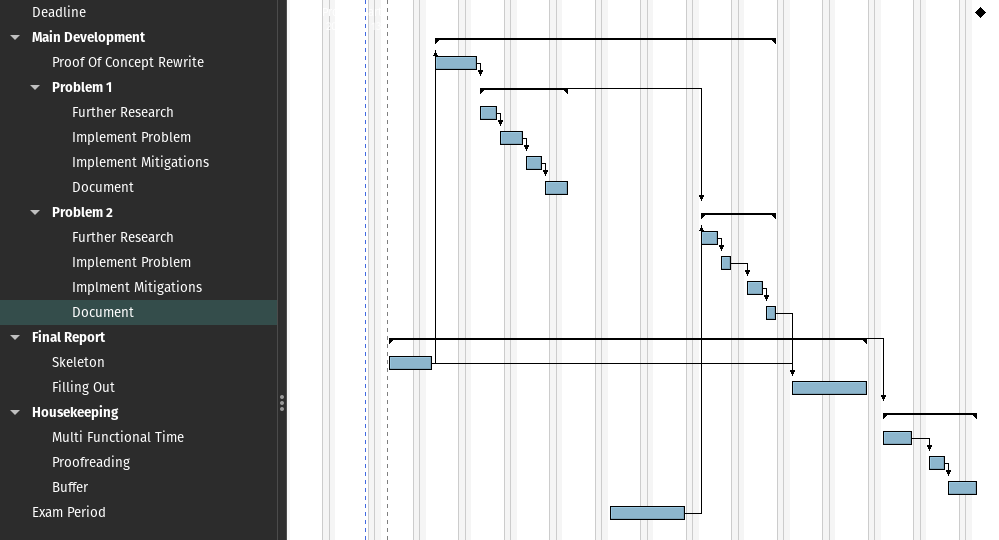
\includegraphics[width=\textwidth]{gantt_post}



\section{Risk Assessment}
\subsection{Personal Issues}

\subsubsection{Description}
This risk entails all personal issues which cause the author to be unable to do work, such as illness.

\subsubsection{Risk Calculations}
\emph{Severity (1-5):} 3 \\
\emph{Likelihood (1-5):} 3 \\
\emph{Overall Risk (1-25):} \textbf{9}

\subsubsection{Mitigation}
As much as possible, the codebase will be designed such that individual sections and modules have minimal dependencies on other sections. This means that, even if the author is unable to work for a period of time, some less critical sections can be omitted without significantly impacting the rest of the project.

\subsection{Hardware Failure - Local Computer}
\subsubsection{Description}
This risk entails a failure on the authors local computer of any kind, such as a graphics card or storage breakage.

\subsubsection{Risk Calculations}
\emph{Severity (1-5):} 4 \\
\emph{Likelihood (1-5):} 2 \\
\emph{Overall Risk (1-25):} \textbf{8}

\subsubsection{Mitigation}
To mitigate storage based failures, the project will be regularly backed up to GitHub. If a core component of the work computer breaks, the author has access to a personal laptop and the Zepler Labs. The deep learning environment along with dependencies is backed up to the authors Google Drive in the form of a docker image, so that switching to a new computer would be a smooth process.

\subsection{Algorithm Fails to Work}
\subsubsection{Description}
This risk describes a situation where the algorithm of swarm learning does not function as well as expected. However, this is very unlikely as swarm learning has been proven to work in numerous papers CITE ME.

\subsubsection{Risk Calculations}
\emph{Severity (1-5):} 5 \\
\emph{Likelihood (1-5):} 1 \\
\emph{Overall Risk (1-25):} \textbf{5}

\subsubsection{Mitigation}
This is not an ideal situation, nevertheless it may be possible to shift the project away from swarm learning and onto federated learning. Federated learning is more commonly used and therefore has more literature, meaning that it is more likely to be an achievable goal to implement it. This would be a last resort though.
	\chapter{Conclusion}
	In conclusion, this paper has shown that SL has the potential to outperform conventional machine learning methods in some cases. While SL presents its own challenges, a plan has been proposed to address these issues and prepare SL for real-world applications. Preliminary testing has been encouraging, and future experiments may provide further evidence of the superiority of SL over conventional machine learning.
	
	\bibliographystyle{ieeetr}
	\bibliography{interim}{}
\end{document}